%4
\section{Konkrete Architektur}
\textcolor{blue}{\textit{In diesem Abschnitt werden die zuvor identifizierten Schnittstellen der Komponenten genauer beschrieben. Im Komponentendiagramm werden daher Abhängigkeiten und Implementierungsbeziehungen beschrieben bzw. ergänzt.
}}
%4.1 Server Software
\subsection{\textit{ServerSoftware}}
\begin{figure}[H]
\centering
\includegraphics[width=1\textwidth]{img/51}
\caption{\textcolor{blue}{Komponentendiagramm für Server}}
\label{KomponentendiagrammKonkret}
\end{figure}
Die \textit{Server} Software tätigt in der nullten Ausbaustufe direkt Aufrufe an den \textit{Robot}, 
um den besten \textit{Robot} für einen \textit{Task} zu ermitteln und einem \textit{Robot} ein \textit{Task} zu geben.

%4.2 Robot Software
\subsection{\textit{RobotSoftware}}
\begin{figure}[H]
	\centering
	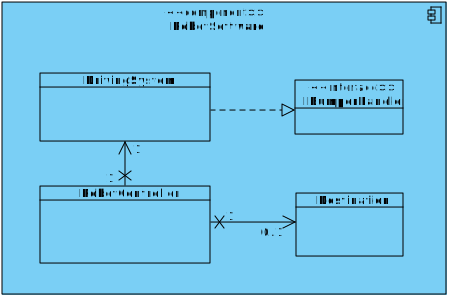
\includegraphics[width=1\textwidth]{img/52}
	\caption{\textcolor{blue}{Komponentendiagramm für Robot}}
	\label{KomponentendiagrammKonkret}
\end{figure}
Die \textit{Robot} Software ist für die Steuerung der \textit{RobotUnit} zuständig. Die von der abstrakten Hardware 
des \textit{Robot} angebotenen gegebenen \textit{Interfaces INorthStar, IBattery, IDrive, IDistanceSensors, IBumper} sowie 
/textit{IBumperHandler} werden dabei von der \textit{Robot} Software für die konkrete Steuerung der \textit{RobotUnit} genutzt.
